\begin{frame}{Bảng Denavit–Hartenberg}
    \begin{columns}
        \column{0.6\textwidth}
        \vspace{-8mm}
        \begin{table}[h]
            \centering
            \caption{Tham số Denavit–Hartenberg.}
            \begin{tabular}{|c|c|c|c|c|}
                \hline
                \textbf{Khớp} & \( \theta_i \) & \( d_i \) & \( a_i \) & \( \alpha_i \) \\
                \hline
                1 & \( \theta_1 \) & \( d_1 \) & \( a_1 \) & \( \alpha_1 \) \\
                \hline
                2 & \( \theta_2 \) & \( d_2 \) & \( a_2 \) & \( \alpha_2 \) \\
                \hline
                3 & \( \theta_3 \) & \( d_3 \) & \( a_3 \) & \( \alpha_3 \) \\
                \hline
                \vdots & \vdots & \vdots & \vdots & \vdots \\
                \hline
                \( n \) & \( \theta_n \) & \( d_n \) & \( a_n \) & \( \alpha_n \) \\
                \hline
            \end{tabular}
        \end{table}
        { \footnotesize
        \begin{equation}
            T_i^{i-1} =
            \left[ \begin{array}{cccc}
            \cos\theta_i & -\sin\theta_i \cos\alpha_i & \sin\theta_i \sin\alpha_i & a_i \cos\theta_i \\
            \sin\theta_i & \cos\theta_i \cos\alpha_i & -\cos\theta_i \sin\alpha_i & a_i \sin\theta_i \\
            0 & \sin\alpha_i & \cos\alpha_i & d_i \\
            0 & 0 & 0 & 1
            \end{array} \right].
        \end{equation}
        }
        \column{0.4\textwidth}
        {\footnotesize 
        \begin{equation}
            \left[ P_x^i, P_y^i, P_z^i, 1 \right]^T = T_i^{i-1} \left[ P_x^{i-1}, P_y^{i-1}, P_z^{i-1}, 1 \right]^T.
        \end{equation}
        }
        \begin{figure}
            \centering
            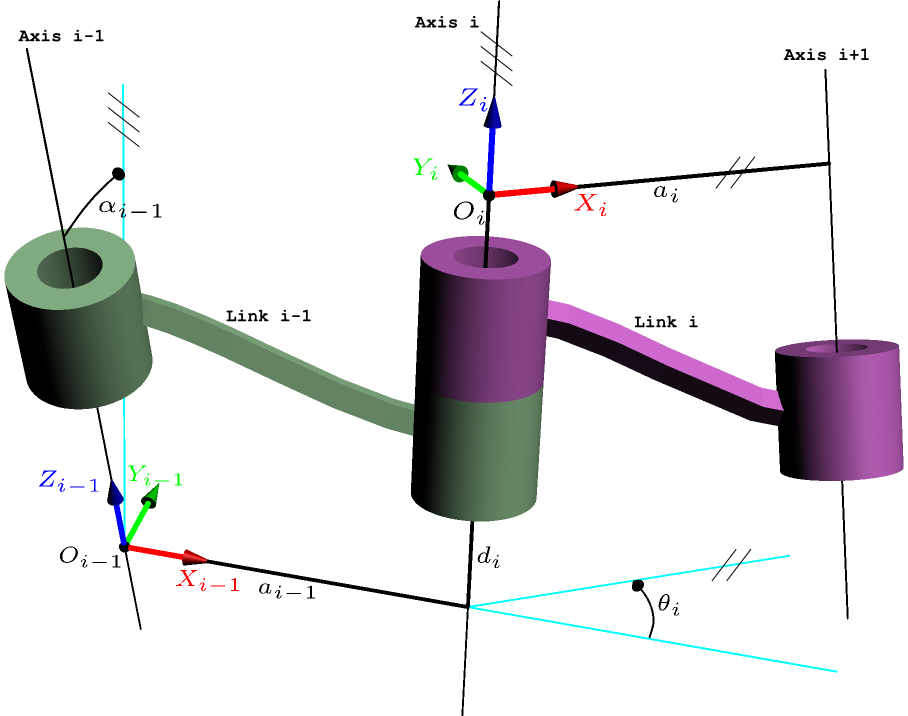
\includegraphics[width=0.8\linewidth]{Figures/DHParameter.png}
            \caption{Các tham số biến khớp để xây dựng bảng Denavit-Hartenberg \cite{craig2011introduction}.}
            \label{fig:Denavit-Hartenberg}
        \end{figure}
    \end{columns}
    
\end{frame}